\documentclass[hyperref={pdfpagelabels=false}]{beamer}

\let\Tiny=\tiny

\usepackage[brazilian]{babel}
\usepackage[T1]{fontenc}
\usepackage[utf8]{inputenc}

\title[\LaTeX{}]{\LaTeX{} Workshop}
\subtitle{Mini Curso de Introdução ao \LaTeX{}}
\author[ROSA]{Wanderson Henrique Camargo Rosa}
\institute[UNISINOS]{
Centro de Ciências Exatas e Tecnológicas\\
Universidade do Vale do Rio dos Sinos (UNISINOS)
}
\date{São Leopoldo, Maio de 2010}
\keywords{latex sbc}

\begin{document}

\begin{frame}
    \maketitle{}
\end{frame}

\section{Histórico}

\begin{frame}{Definição}
    \LaTeX{} é um sistema de composição de textos \cite{oetiker2008}, adequado
    para produção de documentos matemáticos de alta qualidade tipográfica. É uma
    versão especial do \TeX{} que entende comandos próprios \cite{lamport1994} e
    trabalha buscando dividir as funções de formatação do documento e a ordem
    lógica do texto.
\end{frame}

\begin{frame}{Donald Knuth e \TeX{}}
    \begin{itemize}
      \item Cientista da Computação
      \item Análise de Algoritmos
      \item Teoria da Computação
      \item Programação Literária
    \end{itemize}
    \pause{}
    \begin{figure}
        \centering{}
        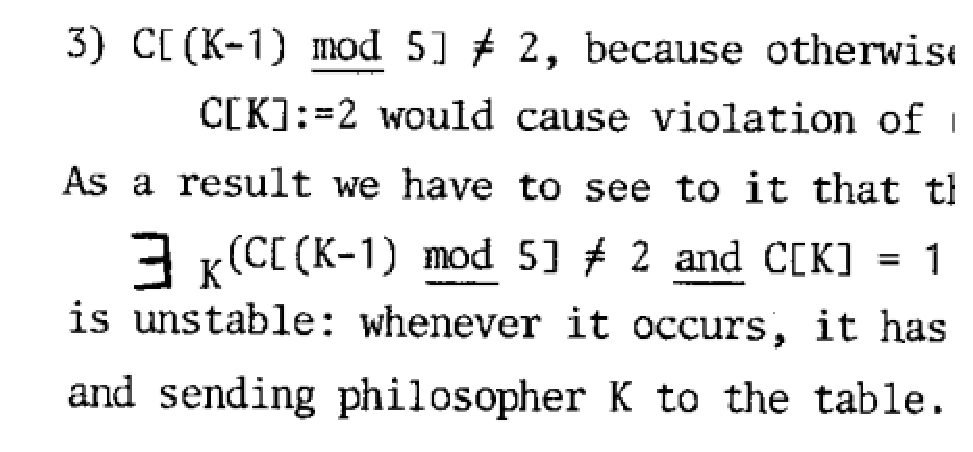
\includegraphics[scale=0.5]{sources/dijkstra.eps}
        \caption{Dijsktra e Ordenação de Processos}
    \end{figure}
\end{frame}

\begin{frame}{Bibliografia}
    \bibliographystyle{plain}
    \bibliography{document}
\end{frame}

\end{document}